\documentclass{report}
\usepackage{graphicx} % Required for inserting images
\usepackage[italian]{babel}
\usepackage{tikz}
\usepackage{hyperref}
\usepackage{amsmath}
\usepackage{xcolor}

\definecolor{darkgreen}{rgb}{0.0, 0.5, 0.0}


\title{Preferenze Privacy degli Utenti}
\date{Parte IV}

\begin{document}

\maketitle

\tableofcontents
\newpage

\chapter{Introduzione}
\subsubsection{Privacy dell'identità degli utenti}
Gli utenti preferiscono restare anonimi o comunque non condividere troppe informazioni quando
operano nel cloud.
Alcuni scenari:
\begin{itemize}
    \item \textbf{Tecniche di comunicazione anonima}
    \item \textbf{Privacy in location-based services} (protezione della location quando sensibile)
    \item \textbf{Attribute-based control access:} è un problema lato server, non ci si basa più su chi un tente sia (l'identità)
        ma sugli attributi che ha (certificati che l'utente presenta)
    \item \textbf{Supporto alle preferenze privacy degli utenti:} problema lato utente; \textit{se mi viene chiesto un documento d'identità, non è che do al server tutto il portafoglio}
\end{itemize}

\noindent Gli utenti potrebbero voler specificare le proprie scelte in termini di politiche del trattamento dei dati, quando:
\begin{itemize}
    \item condividono delle proprie risorse con server esterni (ad esempio i social media)
    \item vengono rilasciate informazioni nelle interazioni digitali (ad esempio lascio la carta di credito per accedere a un servizio)
\end{itemize}

$\rightarrow$ Due aspetti di \textbf{protezione:}
\begin{itemize}
    \item \textbf{rilascio diretto:} regola quando, a chi e perchè un utente rilascia informazioni (es. sto comprando qualcosa)
    \item \textbf{uso secondario:} regola l'uso e la profilazione dei dati da terze parti; anche questo deve essere sotto il controllo dell'utente
\end{itemize}

\section{Rilascio diretto}
La community di ricerca ha sviluppato diverse tecniche per regolare le interazioni
tra \textit{parti sconosciute}, definendo dei
meccanismi di \textbf{attribute-based access control}: consistono in una dipedenza dell'accesso rispetto alle proprietà che un utente ha.
Quello che gli utenti possono fare dipende dagli attributi che possiedono, verificati attraverso i \textbf{certificati}.

L'\textit{access control} non risponde più si o no, ma risponde con i requisiti che il richiedente deve soddisfare per avere l'accesso.
Non solo i server vanno protetti ma anche gli utenti, per questo vanno introdotte delle \textit{\textbf{forme di negoziazione}}.

\subsubsection{Esempio}

Se vogliamo cambiare filosofia, in un sistema aperto (non so chi è l'utente) se
voglio chiedere \textit{"tu soddisfi i requisiti per ottenere l'accesso?"}, 
nascono una serie di problematiche:
\begin{itemize}
    \item come specificare l'autorizzazione
    \item \textit{engine} per il controllo della politica
    \item anche la politica potrebbe essere confidenziale (\textit{non voglio dirti che faccio certi controlli})
    \item come chiedere le cose all'utente
    \item l'utente può avere delle controrichieste (\textit{hai la certificazione per chiedermi la carta di credito? la cripti?})
\end{itemize}

\noindent Questo dialogo deve terminare, deve essere \textbf{corretto} e \textbf{minimale}
nei termini delle informazioni rilasciate; tipicamente vengono usati linguaggi basati sul paradigma logico.

\newpage
\section{Controllo di accesso interattivo}
Il client è colui che richiede il servzio (utente), ha con sé:
\begin{itemize}
    \item \textbf{portfolio} (credenziali e proprietà)
    \item \textbf{stato}
    (stato di informazioni che vuole mantenere)
    \item \textbf{politica}
\end{itemize}

Lo stesso vale per il server, cioè colui che offre il servizio.

\subsection{Interazione senza condizioni da parte del client}
\begin{figure}[ht]
    \centering
    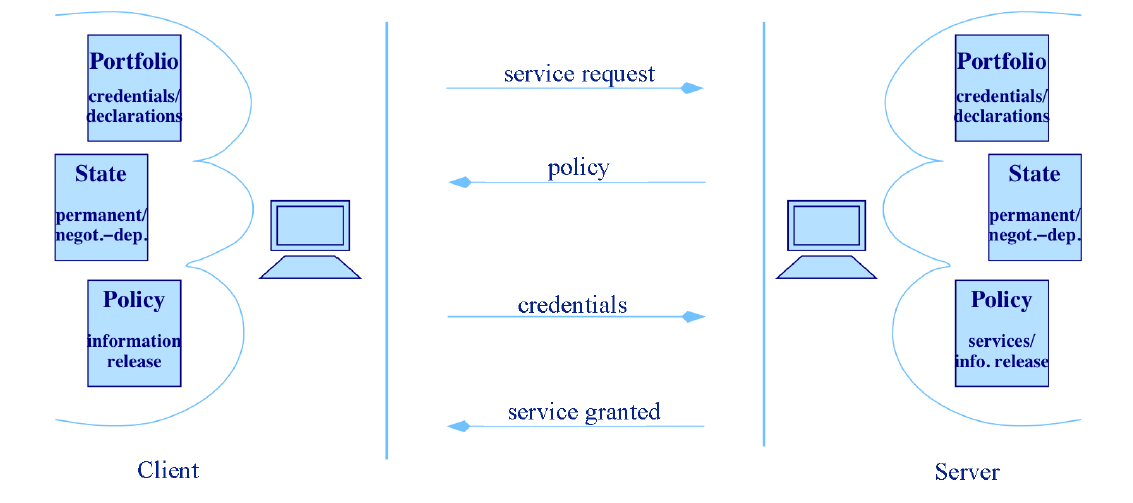
\includegraphics[width=1\linewidth]{images/interactive access control 1.png}
\end{figure}

\noindent La policy del server sta ad indicare ciò che il client deve dimostrare, tramite i certificati, per poter accedere al servzio.

\subsection{Negoziazione \textit{multi-step}}
\noindent In questo caso c'è una negoziazione tra client e server $ \rightarrow $ bisogna stabilire fiducia tra le due parti.

Il server per essere \textit{privacy-friendly} dovrebbe chiedere i dati tutti assieme.

\newpage
\subsection{Interazione a due step}
Per essere \textit{gentili} con l'utente viene fatta una distinzione tra i prerequsiti per l'accesso (necessari ma non sufficenti) e il requisito vero e proprio
con eventuale controrichiesta da parte dell'utente.

\begin{figure}[ht]
    \centering
    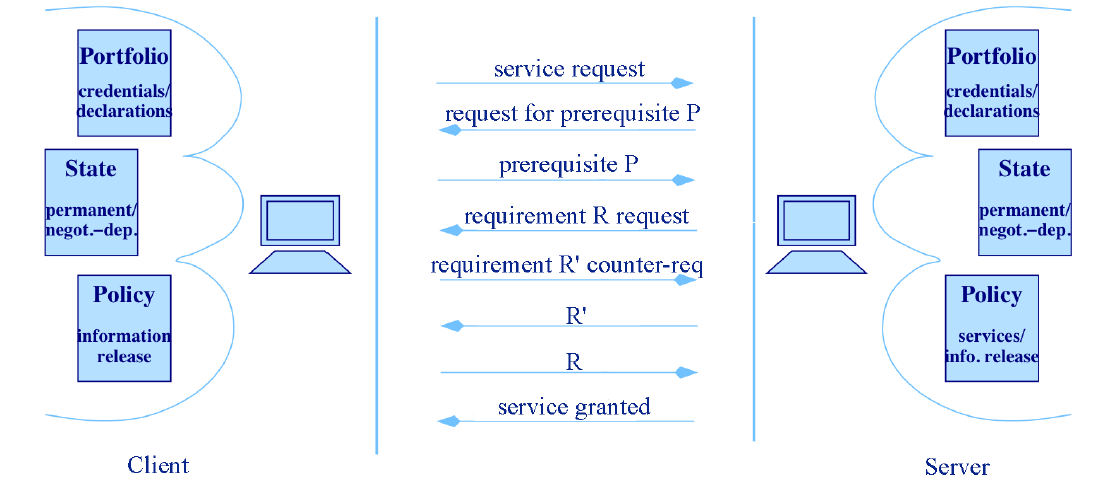
\includegraphics[width=1\linewidth]{images/interactive access control 2.png}
\end{figure}

\subsubsection{Esistenti/emegenti tecnologie di supporto a ABAC}
\begin{itemize}
    \item U-Prove/Idemix: fornisce avanzate tecnologie di gestione dei certificati (i certificati odierni ti permettono di estrapolare dal certificato solo
    l'informazione che voglio fornire all'altra parte, senza fornire tutto il certificato).
    \item XACML: standard di oggi per l'interoperabilità delle politiche di controllo degi accessi
\end{itemize}

\newpage
\section{Preferenze degli utenti}

Le specifiche di controllo degli accessi non sempre si adattano bene con il problema lato utente:
\begin{itemize}
    \item \textcolor{darkgreen}{\textbf{+}} sono espressive, potenti e permettono all'utente di specificare se determinate informazioni possono o non possono essere rilasciate
    \item \textcolor{red}{\textbf{-}} non permettono agli uenti di esprimere che preferirebbero rilasciare determinate informazioni piuttosto che altre, nel contesto in cui ne sia data la possibilità
\end{itemize}

$\rightarrow$ È necessario fornire agli utenti strumenti per definire in modo efficace le preferenze sulla privacy riguardo al rilascio delle loro informazioni

\subsubsection{\textit{Desiderata}}
\begin{itemize}
    \item \textbf{Context-based preferences:} sono disposto a rilasciare un'informazione solo se mi trovo in un certo contesto (\textit{lascio la carta solo quando devo pagare})
    \item \textbf{Forbidden disclosures:} certe cose insieme non le rilascio
    \item \textbf{Associazioni sensibili:} associazioni che sono sensibili, perche sono \textit{quasi identifier} o perché non voglio che tu le veda
    \item \textbf{Limited disclosure:} \textit{se mi chiedi di essere maggiorenne, te lo dimostro ma non voglio dirti la mia età}
    \item \textbf{Instance-based preferences:} \textit{se la mia carta sta per scaedere, preferisco lasciarti quella}
    \item \textbf{History-based peferences:} magari ho già rilasciato qualcosa in passato
    \item \textbf{Proof-based preferences:} \textit{preferisco darti la prova che possiedo un passaporto invece che il passaporto stesso}
    \item \textbf{Non-linkability preferences:} \textit{preferisco lasciarti informzioni che, linkate con terze parti, mi identificano di meno}
\end{itemize}

\noindent Esistono diversi approcci per regolare la preferenza sulla privacy per gli utenti, 
che andiamo a vedere nei prossimi capitoli.

\chapter{Cost-sensitive Trust Negotiation}

\begin{itemize}
    \item Due parti (client e server) interagiscono per stabilire fiducia reciproca tramite lo scambio di credenziali 
    $\rightarrow$ \textbf{\textit{trust negotation protocol}}
    \item Il \textbf{rilascio di una credenziale} è regolato da una politica che specifica dei prerequisiti da soddisfare 
    affinché la credenziale possa essere rilasciata
    \item Credenziali e politiche sono asssociate ad un costo 

    $\rightarrow$ più sono sensibili, più il costo è maggiore 
\end{itemize}

\noindent L'obiettivo è di \textbf{minimizzare i costi totali} di rilascio di credenziali 
e politiche durante la \textit{trust negotation}.

\begin{figure}[ht]
    \centering
    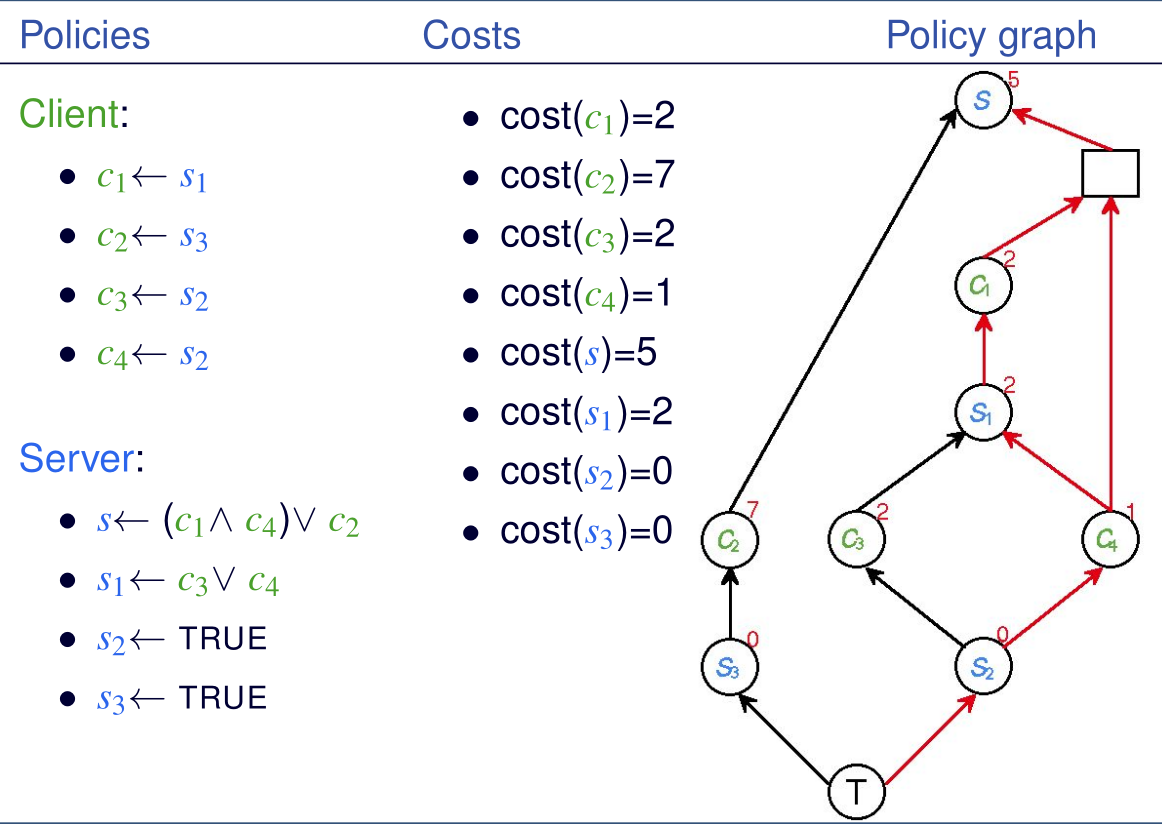
\includegraphics[width=0.83\linewidth]{images/cost-sensitive.png}
\end{figure}

Con $c_1 \leftarrow s_1$ si intende \textit{io rilascio se tu hai}. Il rettangolo nel 
\textit{policy graph} corrisponde ad un AND.

\subsubsection{Conclusioni}

\begin{itemize}
    \item La \textit{cost-sensitive trust negotation} offre un meccanismo per il rilascio delle credenziali 
    in base alla loro sensibilità. Si concentra sulla negoziazione stessa piuttosto che 
    sul controllo da parte dell'utente.
    \item Supporta soltanto specifiche sulle credenziali; \textit{sensitive association} e \textit{forbidden releases} 
    non possono essere specificate.
    \item Questo tipo di approccio (minimizzazione del costo totale) ha un'applicabilità limitata;
    inolte, la combinazione lineare dei costi potrebbe non essere desiderabile.
\end{itemize}


\chapter{Point-based Trust Management Model}
\begin{itemize}
    \item Il server assegna dei \textbf{punti} a ciascuna credenziale
    \begin{itemize}
        \item rappresentano il livello di affidabilità del proprietario 
        \item devono essere tenuti privati
    \end{itemize}
    \item Il server richiede una \textbf{soglia minima di punti totali} per offrire accesso alla risorsa; deve essere tenuto privata
    \item Il client assegna a ciascuna sua credenziale un \textbf{punteggio} (privato), che indica la \textbf{sensibilità} della credenziale
\end{itemize}

$\rightarrow$ l'obiettivo è trovare un sottoinsieme delle credenziali del client che \textbf{soddisfa 
la soglia} stabilita dal server che ha \textbf{valore di privacy minimo} per il client

\newpage
\begin{figure}[ht]
    \centering
    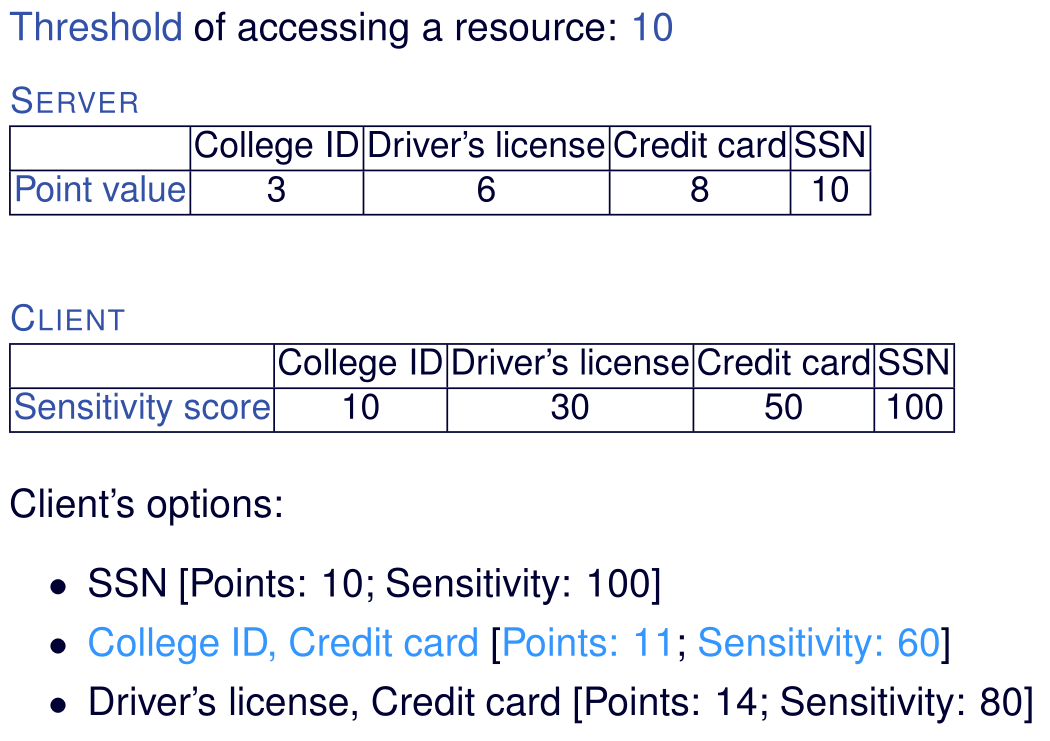
\includegraphics[width=0.85\linewidth]{images/point-based.png}
\end{figure}

\subsubsection{Conclusioni}

\begin{itemize}
    \item Il calcolo della soluzione viene ottenuto convertendo il problema convertendolo 
    al \textit{problema dello zaino}, utilizzando un protocollo sicuro che interagisce con entrambe le parti (client e server), in modo 
    che i punteggi privati non vengano rivelati da una parte all'altra.
    \item Si concentra sulla negoziazione piuttosto che sul controllo da parte dell'utente 
    \item \textit{sensitive association} e \textit{forbidden disclosure} non possono essere specificate
    \item il client e il server devono concordarsi sull'universo dei possibili tipi di credenziali (potrebbe compromettere la confidenzialità delle politiche del server)
\end{itemize}


\chapter{Logic-based Minimal Credential Disclosure}
\begin{itemize}
    \item Le parti sono coinvolte in una \textit{trust negotiation} nella quale il rilascio di
    credenziali è regolato da politiche (problema di bilanciare il linguaggio con la difficoltà delle regole)
    \item Ogni credenziale è un \textbf{singolo attributo}
    \item Combinando le politiche si ottengono diversi \textbf{\textit{negotiation paths}} (set di credenziali per il rilascio) che soddisfano la negoziazione (sia il server che il client possono chiedere qualcosa)
\end{itemize}

$ \rightarrow $ Si usa l'approccio logico per pemrettere agli utenti di specificare le preferenze sulla privacy e selezionare un \textit{negotiation path}.

\begin{figure}[ht]
    \centering
    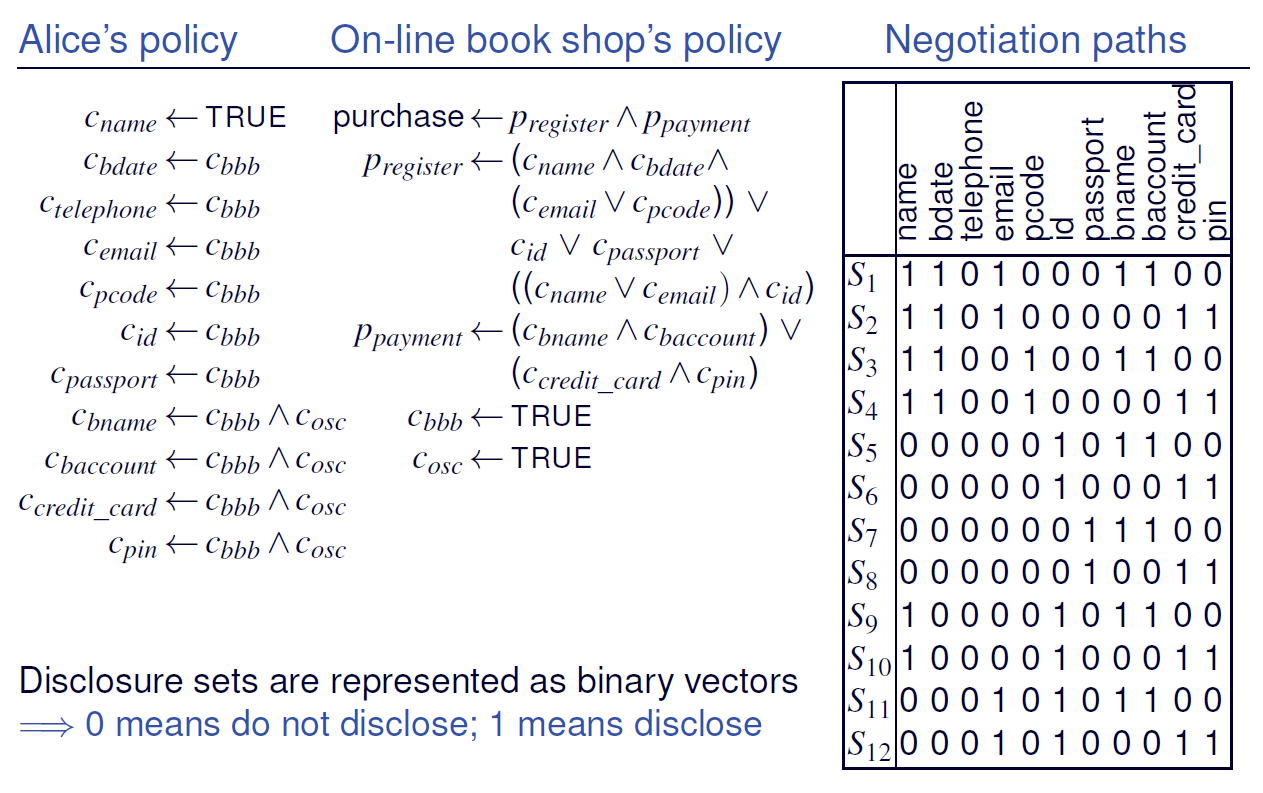
\includegraphics[width=0.85\linewidth]{images/logical-based minimal cred.png}
\end{figure}

Nella colonna di \textit{Alice's Policy} sappiamo che Alice sarà disposta a rilasciare determinate informazioni a patto che la controparte abbia determinati certificati.

\noindent Ciascuna delle righe di \textit{negotiation paths} corrisponde a un possibile rilascio di credenziali al server, con lo scopo di soddisfare \textit{purchase}.
Ogni strategia può essere vista come un vettore binario.

\begin{itemize}
    \item Preferenza di default: non rilasciare una credenziale è meglio che rilasciarla.
    \item I set di rilascio sono confrontati secondo la \textbf{Pareto composition} ($>_P$): 
    
    $ S_i $ domina $ S_j $ se $ S_i $ ha valori migliori o uguali di $ S_j $, ripsettano le preferenze di rilascio delle credenziali ed
    è strettamente migliore rispetto ad almeno una credenziale (rilascia qualcosa in meno)
\end{itemize}
\begin{figure}[ht]
    \centering
    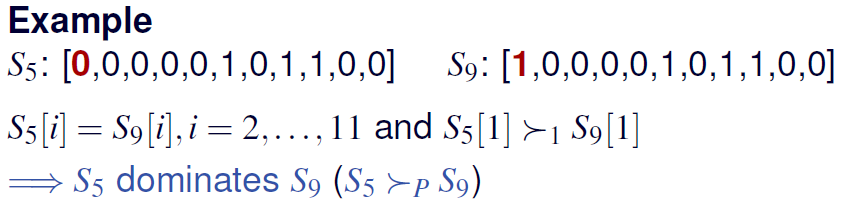
\includegraphics[width=0.85\linewidth]{images/Pareto.png}
\end{figure}

La gerarchia specifica le preferenze di rilascio delle credenziali ($c_i \rightarrow c_j$ signifca che preferiamo rilasciare $ c_i $ rispetto a $ c_j$)
\begin{figure}[ht]
    \centering
    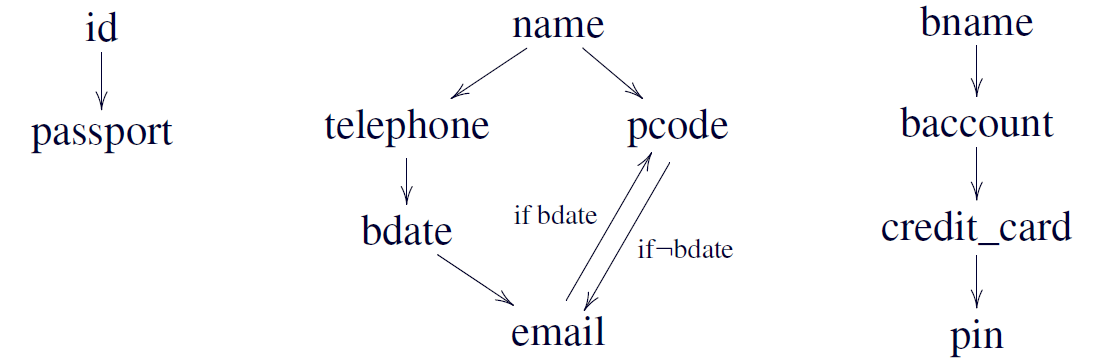
\includegraphics[width=0.85\linewidth]{images/Gerarchia.png}
\end{figure}

È possibile esprimere preferzne condizionate in relazione a cosa ho rilasciato precedentemente.

\begin{figure}[ht]
    \centering
    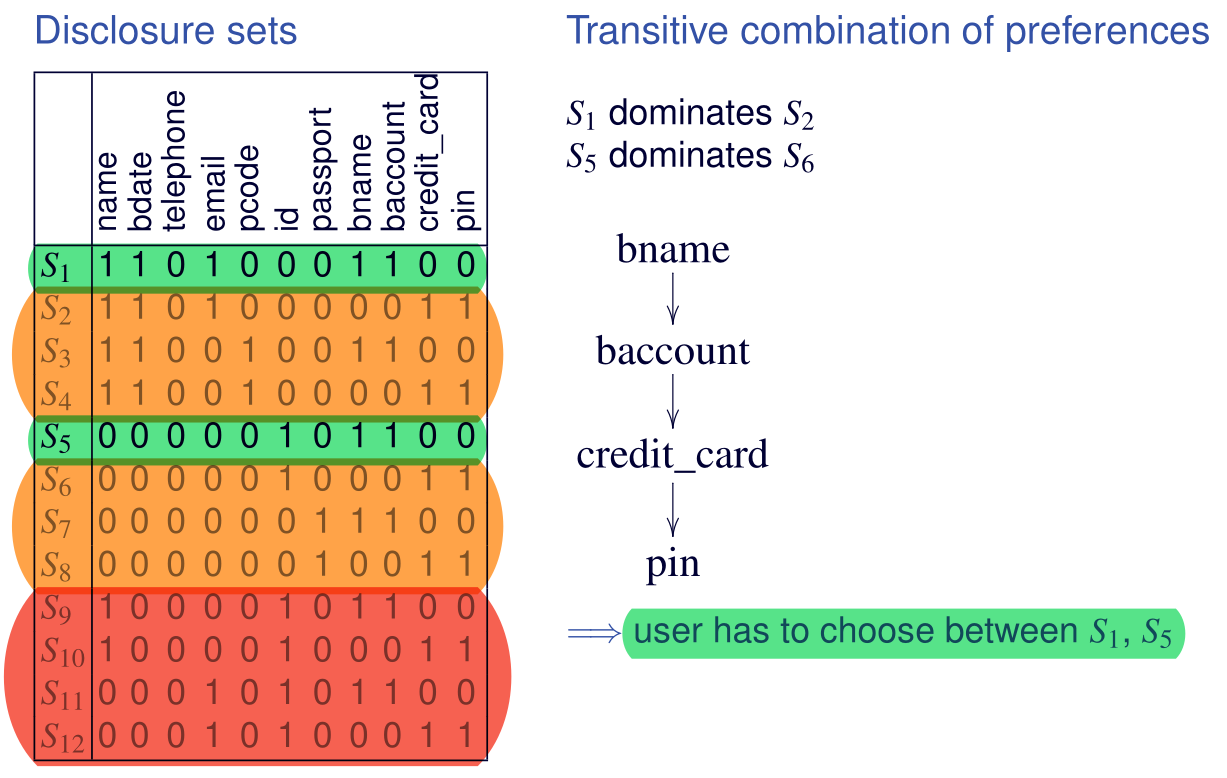
\includegraphics[width=1\linewidth]{images/logic-ex.png}
\end{figure}

Le righe arancione vengono scartate sulle preferenze degli utenti; le righe rosse 
sono scartate perché rilasciano più informazioni di quelle necessarie.

\newpage
\subsubsection{Conclusioni}
\begin{itemize}
    \item Gli utenti sono coinvolti nella scelta del disclosure set
    \item Vengono assunti solo attributi (non si ragiona in termini di credenziali)
    \item La specifica di preferenze su gruppi di attributi non è sempre facile
    \item Credenziali \textit{possession-sensitive} non sono considerate
    \item \textit{Forbidden releases} non sono supportati
\end{itemize}

\chapter{Privacy Preferences in Credential-based Interactions}

\subsubsection{Obiettivo}
Abilitare gli utenti a regolare efficientemente il rilascio delle loro proprietà è credenziali 
\begin{itemize}
    \item Identificare i requisiti e i concetti che necesitano di catturati
    \item Organizzare le proprietà e credenziali dell'utente nel \textit{\textbf{user portofolio}}
    \item Permettere all'utente di specificare quanto valuta le componenti del \textit{portfolio} 
\end{itemize}

\section{Client porfolio}
Le informazioni del client formano il  \textit{Client portfolio}; è composto da:
\begin{itemize}
    \item \textbf{Credenziale:} certificato rilasciato e certificato da una terza parte; 
    \begin{itemize}
        \item certifica delle proprietà
        \item ha un tipo, identificatore e un'entità che la rilascia
    \end{itemize}
    \item \textbf{Dichiarazione:} credenziale \textit{self-signed} (rilasciata da me stesso)
\end{itemize}

\noindent Si definisce una \textbf{gerarchia di astrazione} di tipi di credenziali.

\begin{figure}[ht]
    \centering
    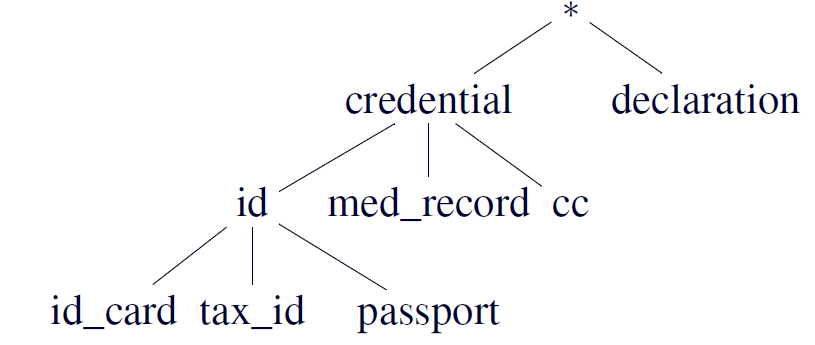
\includegraphics[width=0.7\linewidth]{images/client portfolio.png}
\end{figure}

\subsection{Client Portfolio - Proprietà}
\begin{itemize}
    \item \textbf{Credential-indipendent:} il valore è sempre lp stesso indipendentemente da chi lo rilascia
    \item \textbf{Credential-dipendent:} il valore dipende dalla credenziale che lo certifica (es: passaporto)
    \item \textbf{Atomic:} rilasciate unitamente; se rilasciata, tutte le sue proprietà vengono rilasciate 
    \begin{figure}[ht]
    \centering
    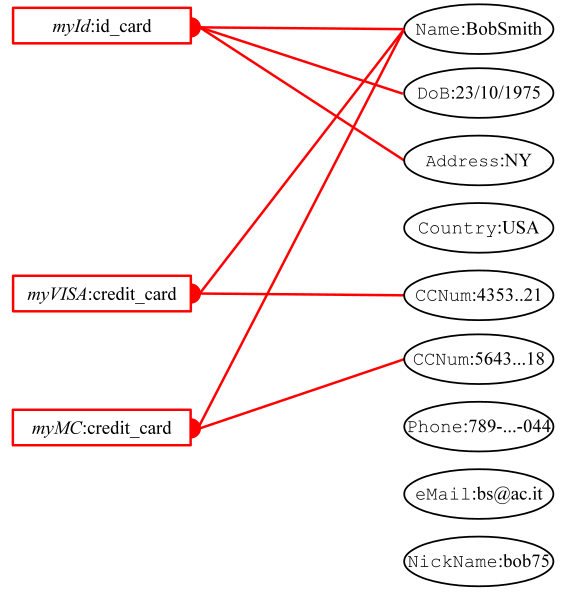
\includegraphics[width=0.6\linewidth]{images/ atomic.png}
    \end{figure}
    \item \textbf{Non-atomic:} le proprietà possono essere rilasciate disgiuntamente 
    \begin{figure}[ht]
        \centering
        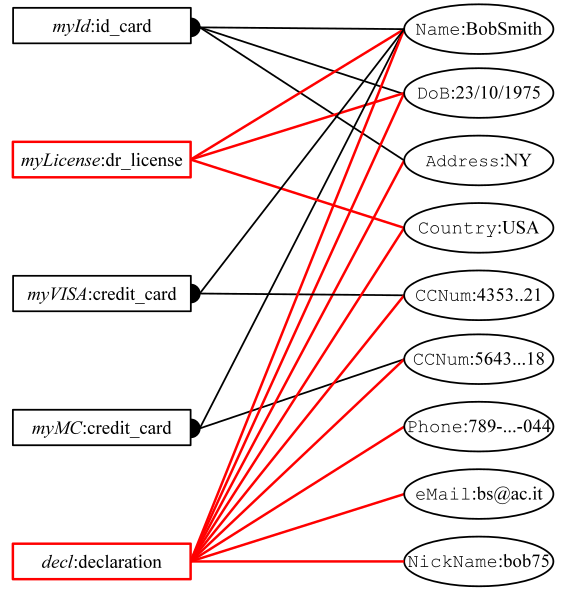
\includegraphics[width=0.6\linewidth]{images/non-atomi.png}
    \end{figure}
\end{itemize}

\newpage
\subsection{Disclosure}
Un rilascio è un sottoinsieme del \textit{portfolio} del client che soddisfa:
\begin{itemize}
    \item \textbf{Certificabilità:} ogni proprietà è certificata da una credenziale
    \item \textbf{Atomicità:} se la proprietà di una credenziale atomica è rilasciata, tutte le sue proprietà sono rilasciate 
\end{itemize}

\section{Sensibilità del portfolio}

\begin{itemize}
    \item Diverse componenti del portfolio potrebbero avere sensibilità diverse
    
    $\rightarrow$ l'utente potrebbe preferire il rilascio di una sulle altre
    \item I requisiti di privacy vengono espressi usando delle \textbf{etichette di sensibilità:} 
    \begin{itemize}
        \item stabiliscono una gerarchia con ordine parziale $\geq$
        \item e una composizione additiva dei valori $\oplus$ 
        
        $\rightarrow$ la composizione di due etichette $\lambda_1 \oplus \lambda_2$ è anch'essa un'etichetta di sensibilità 
    \end{itemize}
    \item Assumiamo che le etichette abbiano valori interi, e la loro composizione si ottiene attraverso l'operatore $+$
\end{itemize}

\newpage
\subsection{Sensibilità di proprietà e credenziali}
Specificano come il client valuta la sensibilità delle informazioni nel suo portfolio.

\begin{figure}[ht]
    \centering
    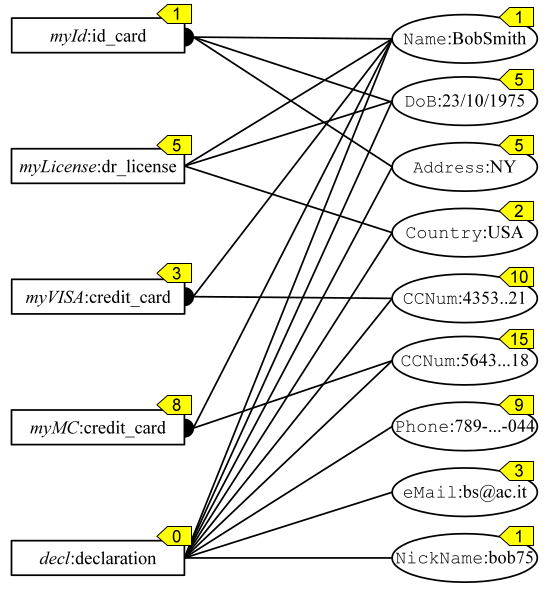
\includegraphics[width=0.75\linewidth]{images/cred-prop-sens.png}
\end{figure}

\begin{itemize}
    \item A sinistra viene riportata la sensibilità associata all'\textbf{esistenza della credenziale};
    \textit{che il mio nome sia su una carta d'identità non ha lo stesso valore di una denuncia penale}
    \item A destra viene riportata la sensibilità della \textbf{proprietà presea singolarmente}
\end{itemize}

\newpage
\subsection{Sensibilità delle associazioni}
\begin{figure}[ht]
    \centering
    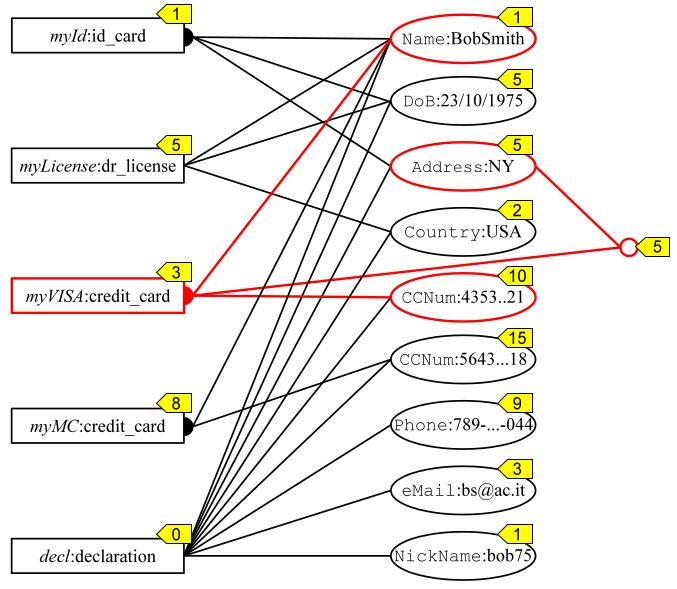
\includegraphics[width=1\linewidth]{images/sens-ass-1.png}
\end{figure}
In questo caso viene riportata la sensibilità dell'associazione della credenziale 
\textit{carta di credito} con \textit{indirizzo}; in questo caso sto aggiungendo 
delle informazioni $\rightarrow 5$ rappresenta la sensibilità che devo aggiugere dovuta all'associazione

\subsubsection{Esempio}
Il mio \textit{nome} e \textit{nickname} presi singolarmente non sono sensibili; la loro 
associazione però è sensibile.

\newpage
\begin{figure}[ht]
    \centering
    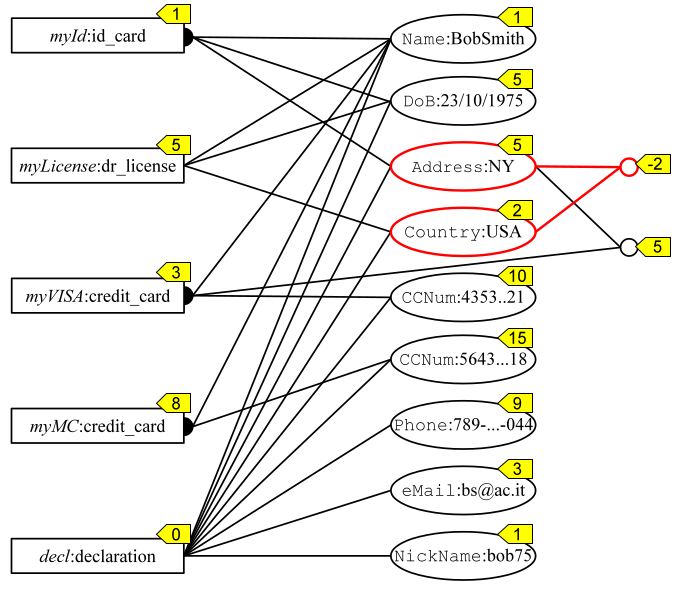
\includegraphics[width=1\linewidth]{images/sens-ass-2.png}
\end{figure}
In questo caso sto aggiungendo un'informazione (\textit{country}) che in realtà non mi 
dice niente, dato che una implica l'altra

$\rightarrow $ togliamo $2$ perché questa associazione non mi dice niente di nuovo

\newpage
\subsection{Disclosure Constraints}
\begin{figure}[ht]
    \centering
    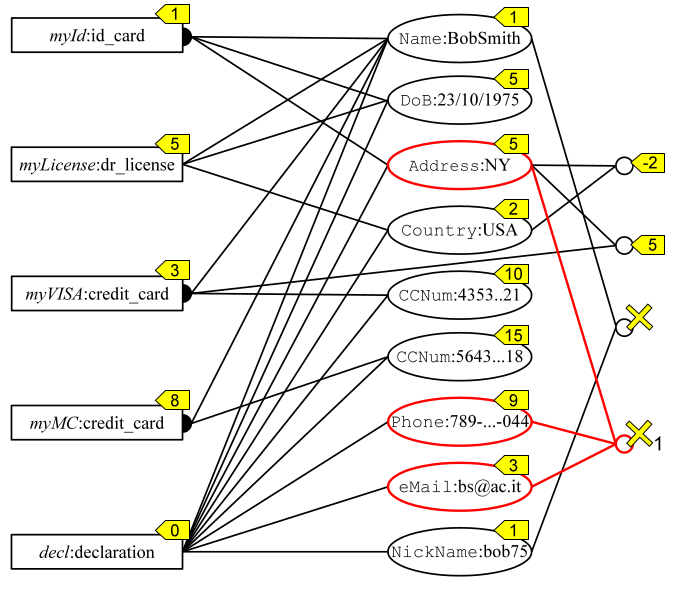
\includegraphics[width=1\linewidth]{images/disclosure-constraints.png}
\end{figure}
Permettono di indicare quegli elementi il cui rilascio deve essere controllato.

\begin{itemize}
    \item La prima $X$ indica che il rilascio dell'associazione è \textbf{proibita}; \textit{non voglio che siano rilasciate insieme}
    \item La seconda $X$ indica un rilascio \textbf{limitato}; al massimo $n$ (in questo caso $n=1$) elementi 
    dell'associazione possono essere rilasciati (in questo caso al massimo $1$ tra \textit{address, phone, email})
\end{itemize}

\noindent Un rilascio è \textbf{valido} se nessun \textit{disclosure constraint} viene violato.  





\end{document}